\section{A Discrete Version}
\label{sec:discrete}

In this section, we use the Gauss-Bonnet theorem to derive
a definition of discrete curvature. We discuss how discrete curvature
is used to improve meshes that are generated by scanning.
We then prove a discrete version of the Gauss-Bonnet theorem.

Consider a triangulated polygonal surface $S$ with boundary $\partial(S)$.
The boundary is a one dimensional piecewise linear curve in $\R^3.$
As with polygons in the plane, at each vertex $v\in \partial(S)$ 
we have an exterior angle.

The interior angle might consist of many triangles.
Let $F_v$  denote the set of faces incident to $v$ and let
$\alpha_f$ denote the angle in face $f$ at $v$.
The \EMPH{discrete geodesic curvature}
of $v$  is
$$k_{g}(v)= \pi-\sum_{f\in F_v}\epsilon_f.$$
See \figref{discrete-geodesic} for an illustration.
Notice that if $v$ lies on a straight line, then $\sum_{i}\alpha_f=\pi$
and the curvature is zero as we would expect.
The word geodesic is used because we are measuring how close
a curve is to being straight with respect to the surface we are on.


\begin{figure}[htb]
\centering
	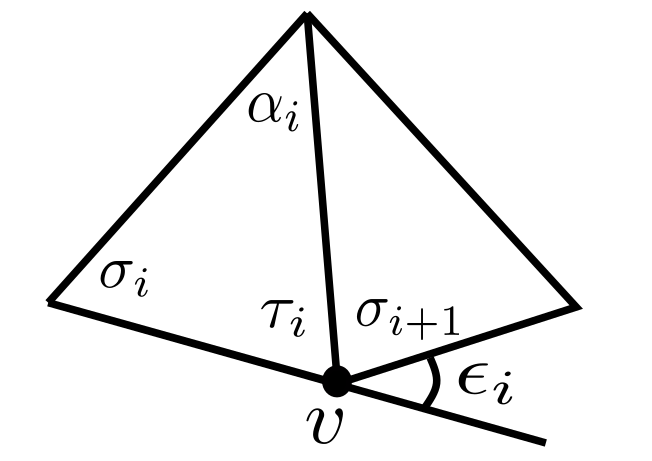
\includegraphics[width=.3\textwidth]{curvature/discrete-geodesic}
	\caption{The discrete geodesic curvature at a vertex $v$ on the boundary
	of a surface is given by the exterior angle $\epsilon$.}
	\label{fig:discrete-geodesic}
\end{figure}



A geometric definition of discrete Gaussian curvature is the following:
\begin{definition}[Discrete Gaussian curvature]\label{def:discrete-curvature-vertex}

The discrete \EMPH{Gaussian curvature} at a vertex $v$ is the area on the unit 
sphere bounded by a spherical polygon whose vertices are the unit normals of 
the faces around $v$.

\end{definition}

If a vertex is on a flat surface, then the unit normals are all pointed
in the same direction and the Gaussian curvature is zero.

\begin{figure}[htb]
\centering
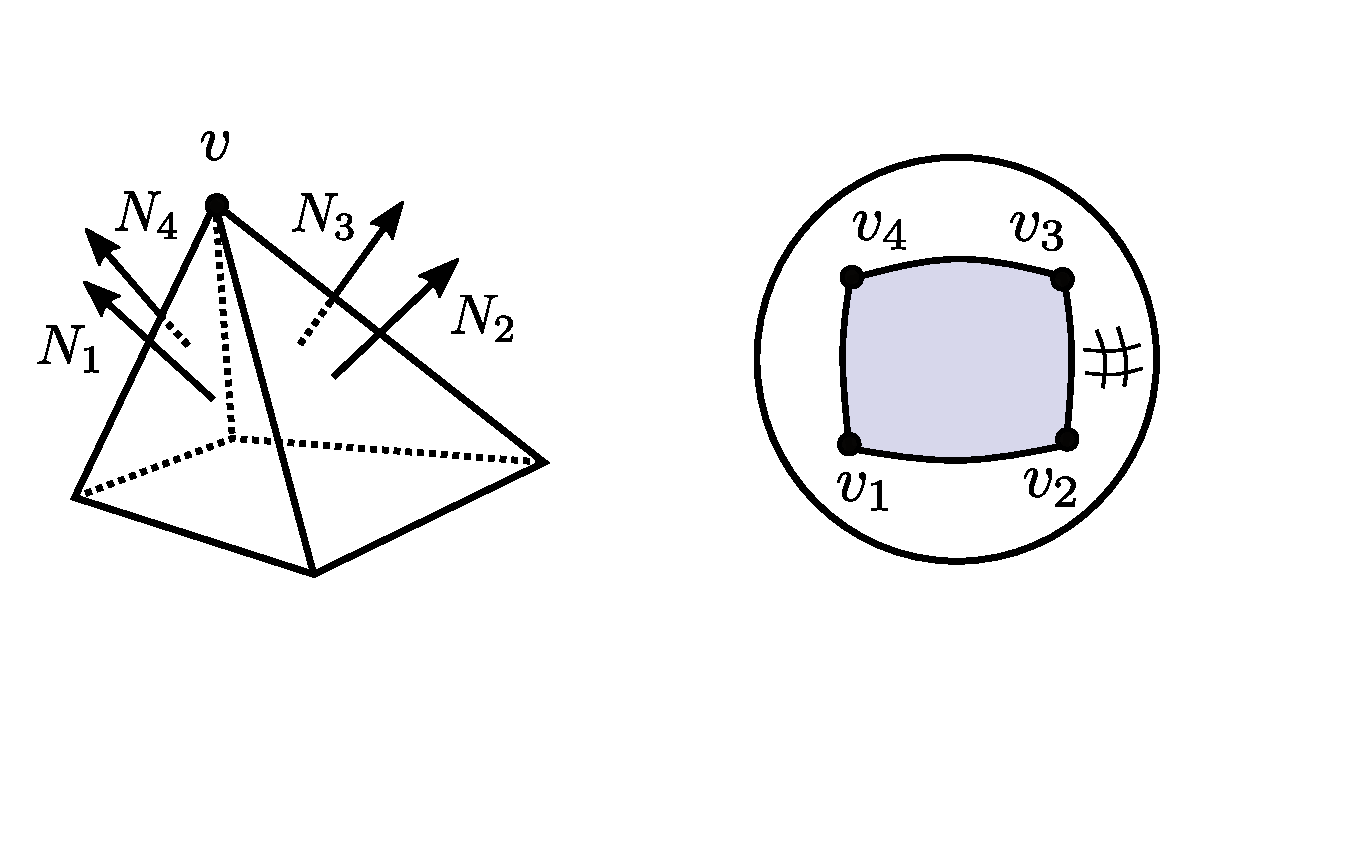
\includegraphics[width=.5\textwidth]{curvature/discrete-curvature}
\caption{Consider the vertex $v$ in the figure on the left. The curvature of $v$
is the area on the sphere shown on the right. We rotated the sphere
in order to see the entire polygon.}
\label{fig:discrete-curvature}
\end{figure}


Let $\alpha_i$ denote the angle of a triangle incident to $v$, 
we next show that the interior angle of the polygon $\beta_i$ on the 
sphere is supplementary $\alpha_i$.

\begin{equation} \label{eqn:switcheroo}
\beta=\pi-\alpha.
\end{equation}
Notice that the edge between two faces
on a triangulated surface
is perpendicular to the normal vectors of the faces.
So, the line connecting two normal vectors will intersect the edge between the vectors 
at right angles. See \figref{switcheroo}.


\begin{figure}[htb]
\centering
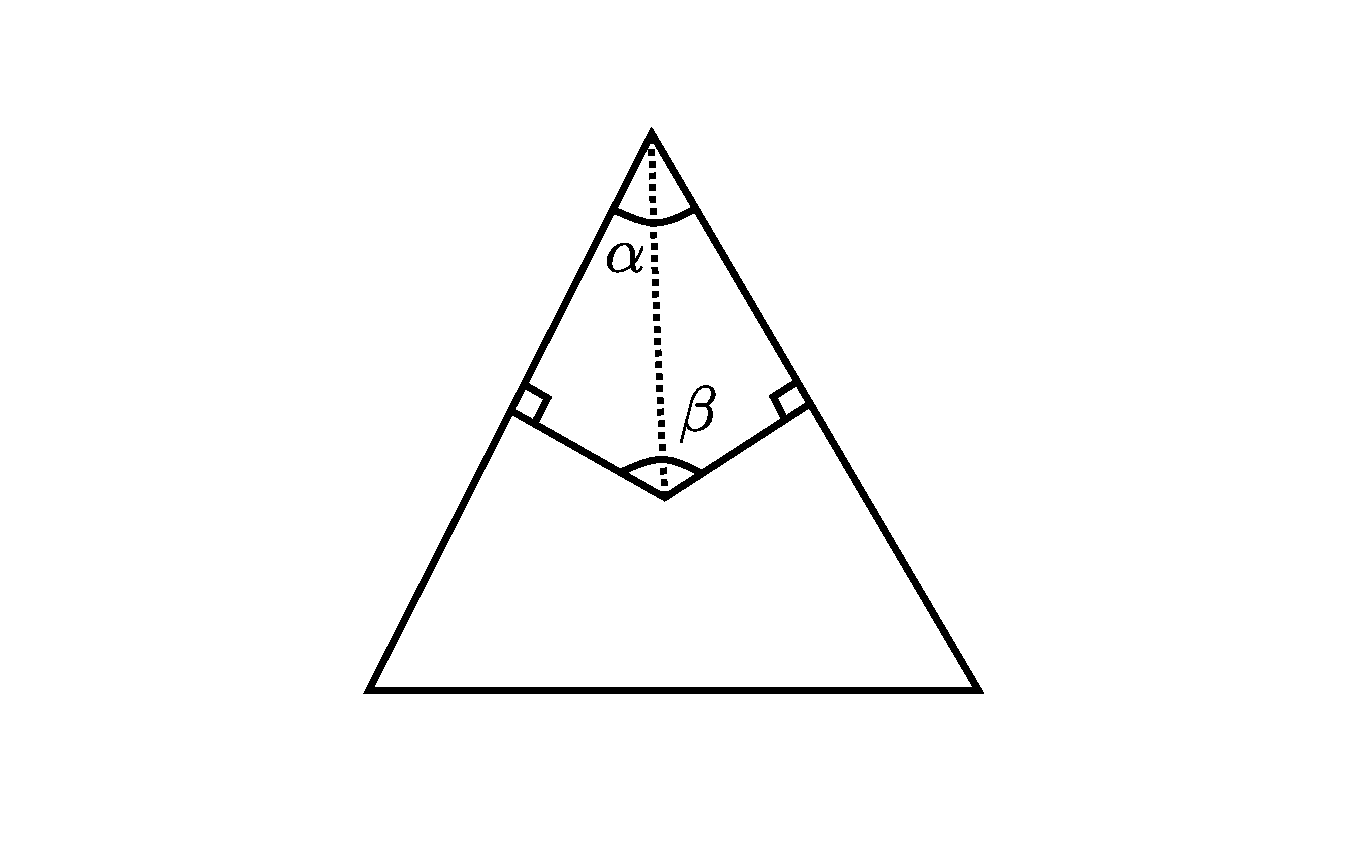
\includegraphics[width=.25\textwidth]{background/switch-angles}
\caption{The relationship between the angles incident to a vertex and
the interior angles of the area polygon on the sphere.}
\label{fig:switcheroo}
\end{figure}



This gives a  formula for computing the curvature at an interior vertex.
The \EMPH{angle defect} at a vertex $d(v)$ is the difference between $2\pi$ and
the sum of the incident angles.  Let $F_v$ denote the faces containing $v$  
and let $\alpha_f$  denote the interior  angle of face $f$ at $v$, then
\begin{equation} \label{eqn:defect}
d(v):=2\pi -\sum_{f\in F_v}\alpha_f.
\end{equation}
Since $\beta_i=\pi-\alpha_i$,
we can use our formula for the area of a polygon on the sphere,
\eqnref{sphere-area}, to compute the Gaussian curvature at $v$
by
$$K(v)=2\pi -n\pi+\sum_{i}^n \beta_i=2\pi-n\pi +\sum_{i}^n (\pi-\alpha_i) =2\pi-\sum_i^n\alpha_i=d(v)$$
 and the
 angle defect is equal to the discrete curvature in \defref{discrete-curvature-vertex}
 and in \eqnref{discrete-gaussian}.







Combining the above definitions  we have

\begin{theorem}[The Discrete Gauss-Bonnet Theorem] \label{thm:g-b-d}

If $S$ is a triangulated surface with  boundary $\partial S$ then

$$\sum_{v\in V_{int}} K(v) + \sum_{v\in V_{\partial S}} k_g(v) = 2\pi \chi(S)$$
where $K(v)$ is the discrete Gaussian curvature
of a vertex, $k_g(g)$ is the discrete geodesic curvature,  and
$\chi$ is the Euler characteristic.
\end{theorem}



\section{Removing Noise From A Scanned Object}
\label{sec:removing}



Meshes that are obtained by scanning real objects contain noise.
Most meshes that are generated by scanning require a complete
remeshing \cite{remeshing-2003}.
As a first step in remeshing, the curvature at each
vertex needs to be estimated.

In \cite{mmsb-2003}, Meyer et al., define the gaussian curvature operator
to estimate the curvature at each vertex. Their operator is 
based on a simple application of the Gauss-Bonnet theorem.
The central idea is to cut a disk around each vertex that does not contain
any other vertices. Then, all Gaussian curvature in the removed
disk is occurs at the vertex of interest.

We associate an area around each vertex$v$. 
For each triangle incident to $v$, if the interior 
angle at $v$ is non-obtuse, mark the circumcenter of the triangle
and if the interior angle is obtuse, make the mid point of the edge
opposite of $v$. See \figref{mixed-area} for an illustration.
Denote the area of this polygon by $A_m.$


\begin{figure}[htb]
\centering
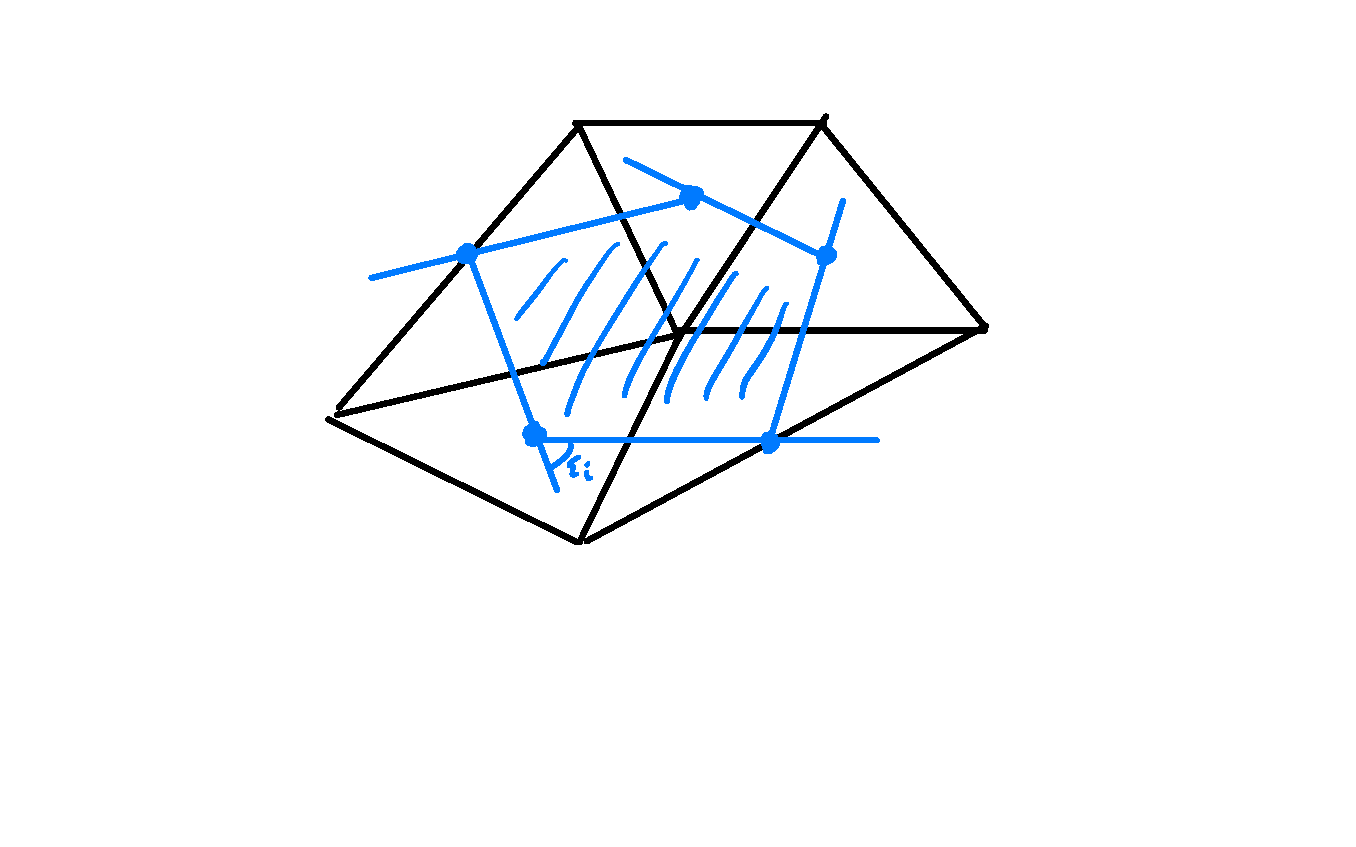
\includegraphics[width=.3\textwidth]{meshes/mixed-area}
\caption{The area $A_m$ associated with a vertex $v$.}
\label{fig:mixed-area}
\end{figure}


Then, since we are considering a closed two-disk $A$ we have $\chi(A)=1$.
Let $F_v$ denote the number of faces incident to $v$, 
then by the Gauss-Bonnet theorem we have

$$\int \int_{A_m}K dA +\sum_i^{F_v} \epsilon_i=2\pi$$
where the sum is over the faces incident to $v$.
The Gaussian curvature operator at a vertex $v$ is defined
to be
$$K(v)=\left( 2\pi -\sum_i^{F_v}\epsilon_i\right)/ A_m.$$

The experiments in \cite{mmsb-2003} found that the average
percent error did not exceed $1.3\%$ when using this operator.



\subsection{A Combinatorial Proof}
\label{sec:proof}


We present a proof of the Gauss-Bonnet theorem similar to the proof given by Upadhyay \cite{upadhyay2015}.
First, we consider the case where our surface does not have a boundary.
We then extend this case to surfaces with boundary.
\begin{theorem}[Discrete surfaces without boundary]\label{thm:g-b-discete-bdy}
For a triangulated surface $S$ without boundary
$$\sum_{v\in V} K(v)=2\pi \chi(S)$$
where $K(v)$ is the discrete curvature.
\end{theorem}

\begin{proof}

For each vertex $v$ in $S$,
let $deg(v)$ denote the number of edges incident to $v$, let $\alpha_1,\alpha_2,\ldots,\alpha_{\deg{(v)}}$ denote the angles
containing $v$ and let $\xi_i=\pi-\alpha_i$ for each $i$.
By \eqnref{discrete-curvature-complement-angle}, 
the discrete Gaussian curvature at a $v$ is
 $$K(v)=(2-\deg{(v)})\pi +\sum_{i=1}^{\deg{(v)}} \xi_i.$$
Summing over all vertices in $S$ gives
$$\sum_{v\in V} K(v)=\sum_{v\in V}2\pi - \sum_{v\in V}\deg{(v)}\pi+\sum_{v\in V}\sum_{i=1}^{\deg{(v)}} \xi_i.$$
The first term on the right hand side is $2\pi |V|$. Each edge is incident with two vertices, so the second term is $2\pi |E|$. 
In the third term, we rewrite $\xi_i$ as $\pi-\alpha_i$.

$$ \sum_{v\in V}\sum_{i=1}^{\deg{(v)}} \beta_i= \sum_{v\in V}\sum_{i=1}^{\deg{(v)}} (\pi-\alpha_i).$$
We can reorganize this sum as follows, instead of summing the angles around each vertex we can sum the angles in each face.
Each angle in $S$ is still being counted exactly once. 
Since each face is a triangle, this gives
$$\sum_{v\in V}\sum_{i=1}^{\deg{(v)}} (\pi-\alpha_i)=\sum_{f\in F}\sum_{i=1}^3(\pi-\alpha_i).$$
Since each face is a triangle the sum of the three angles is $\pi$,
so $\sum_{i=1}^3(\pi-\alpha_i)=3\pi-\pi=2\pi.$
Thus, $$\sum_{v\in V} K(v)=2\pi |V|-2\pi |E|+2\pi |F|=2\pi \chi(S)$$ as desired.
\end{proof}

Next, we extend the above proof to the case where $S$ has a boundary
by gluing a copy of $S$ to itself along the boundary.

\begin{theorem}[Discrete surfaces without boundary]\label{thm:g-b-discete}
For a combinatorial surface $S$ with boundary

$$\sum_{v\in S_{\text{int}}} K(v)+\sum_{v\in\partial S}k_g(v)=2\pi \chi(S)$$
where $K(v)$ is the discrete curvature and $k_g(v)$ is the discrete geodesic curvature.
\end{theorem}

\begin{proof}
Take a copy of $S$ and attach it to itself along the boundary.
This creates the surface $2S$ without boundary. Notice,
when we copy $S$ we create two copies of the boundary, and when
we glue we remove one copy of the boundary.
Thus, $$\chi(2S)=2\chi(S)-\chi(\partial S).$$
Since, $\partial S$ is piecewise linear the number of vertices and
edges are equal and there are no faces, so $\chi(\partial S)=0$
and 

\begin{equation} \label{eqn:glue}
\chi(2S)=2\chi(S).
\end{equation}
For $v$ a vertex on the boundary, $k_g(v)$ is half
the discrete Gaussian curvature of $v$ in $2S.$
Thus,

$$\sum_{v\in 2S}K(v)=2\left(\sum_{v\in S_{\text{int}}}K(v)+\sum_{v\in \partial S} k_g(v)\right) =2\pi  \chi(2S).$$
Applying \eqnref{glue},

$$\sum_{v\in S}K(v)+\sum_{v\in \partial S} k_g(v)=2\pi  \chi(S)$$
as desired.

\end{proof}